\documentclass{article}

\usepackage{cancel}
\usepackage{tikz}
\usepackage{amsmath}
\usepackage{geometry}
\usepackage{graphicx}
\usepackage{amsfonts} 
\usepackage{verbatim}
\usepackage{mathrsfs}  
\usepackage{lmodern}
\usepackage{braket}
\usepackage{steinmetz}
\usepackage{bookmark}

\hypersetup{
    colorlinks=true,
    linkcolor=black,
}
\tikzset{block/.style = {draw, fill=white, very thick, rectangle, minimum height=1cm, minimum width=2cm}}


\renewcommand{\contentsname}{Indice}

\numberwithin{equation}{subsection}

\title{Appunti di Fondamenti di Telecomunicazioni}
\author{Giacomo Sturm}
\date{AA: 2023/2024 - Ing. Informatica}

\begin{document}

\maketitle

\vspace{10mm}

\begin{center}
    Sorgente del file LaTeX disponibile su \url{https://github.com/00Darxk/Fondamenti-di-Telecomunicazioni}
\end{center}

\clearpage

\tableofcontents

\clearpage

\section{Segnali}

Un segnale è definito come una qualsiasi grandezza fisica che varia nel tempo in maniera deterministica o aleatoria. Può essere un'onda di pressione come la voce, o un onda 
elettromagnetica come segnali wireless e bluetooth. Un segnale è in grado di contenere informazioni come una sequenza di bit. Generalmente un segnale 
analogico viene convertito in digitale come un segnale elettrico tramite un trasduttore, per facilitare la processazione, per poi essere riconvertito in analogico; alcuni 
segnali sono creati direttamente in digitale. Un segnale è definito dalla sua banda, o spettro di banda, che ne determina la capicità di trasmettere informazione. L' 
occupazione in frequenza di un segnale è analoga al numero di bit di un dato digitale. 



Un segnale comune è il segnale voce, definito da un'onda di pressione, per cui è sempre strettamente positivo. Questo segnale è analogico, quindi continuo, ed il suo valoro è 
noto in ogni istante di tempo $t$, e si identifica come $x(t)$. 

\begin{center}
    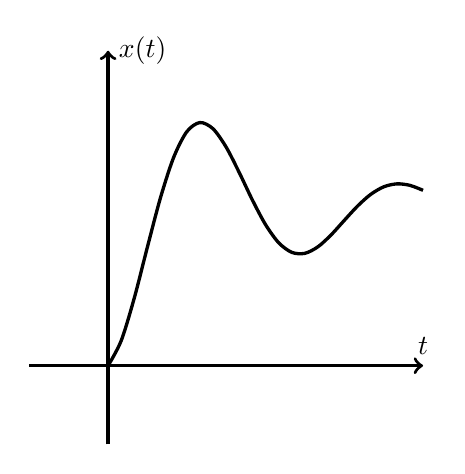
\begin{tikzpicture}[scale=2]
        \draw[->,very thick](-0.5,0)--(2,0)node[above]{$t$};
        \draw[->,very thick](0,-0.5)--(0,2)node[right]{$x(t)$};

        \draw[-,very thick]plot[smooth, domain=0:2](\x,{e^(-\x)*sin((5*\x-pi/2) r)+1});
    \end{tikzpicture}
\end{center}

Campionando un segnale anlogico si crea un segnale digitale, considerando prima alcune condizioni definite dal teroema del campionamento. Per campionare un segnale si estraggono
valori, o campioni, dal segnale analogico ogni intervallo $T$. Il segnale così ottenuto è un segnale discreto $x_n$ o $x[n]$, che presenta un valore ogni multiplo del tempo di campionamenoto $T$ 
scelto. 
\begin{equation*}
    x[n]:=\{x(n\cdot T)\,\forall n\in\mathbb{N}\}
\end{equation*}

\begin{center}
    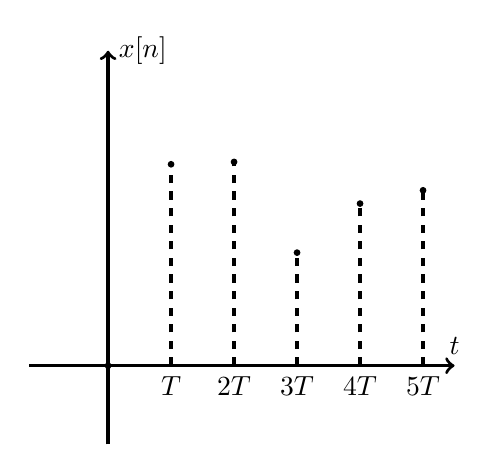
\begin{tikzpicture}[scale=2]
        \draw[->,very thick](-0.5,0)--(2.2,0)node[above]{$t$};
        \draw[->,very thick](0,-0.5)--(0,2)node[right]{$x[n]$};        

        \filldraw[black](0,0)circle(0.5pt);
        \filldraw[black](0.4,1.279)circle(0.5pt);
        \filldraw[black](0.8,1.294)circle(0.5pt);
        \filldraw[black](1.2,0.718)circle(0.5pt);
        \filldraw[black](1.6,1.0294)circle(0.5pt);
        \filldraw[black](2,1.1136)circle(0.5pt);

        \draw[dashed,very thick](0.4,0)node[below]{$T$}--(0.4,1.279);
        \draw[dashed,very thick](0.8,0)node[below]{$2T$}--(0.8,1.294);
        \draw[dashed,very thick](1.2,0)node[below]{$3T$}--(1.2,0.718);
        \draw[dashed,very thick](1.6,0)node[below]{$4T$}--(1.6,1.0294);
        \draw[dashed,very thick](2,0)node[below]{$5T$}--(2,1.1136);
    \end{tikzpicture}
\end{center}

Questi valori vengono poi convertiti in digitale assegnando un certo numero di bit per rappresentare l'intervallo massimo di valori descritti dal segnale. Questo processo 
viene chiamato quantizzazione, si divide l'intervallo dei valori in piccoli intervalli ognuno con un univoco valore in bit, in modo da convertire tutti i valori in quell'
intervallo in una sequenza di bit. Aumentando il numero di bit, quindi il numero di suddivisioni dell'itnervallo di partenza, aumenta la precisione, ma aumenta anche il costo 
per processare lo stesso segnale. Dopo aver covnertito tutti i valori in una sequenza di bit, questo segnale in bit viene tramesso, ed in seguito decodificato in analogico. 
Spesso i segnali vengono creati in digitale, per cui non è necessario campionare un segnale analogico. 


Campionando un segnale si perdono le informazioni contenute tra i campioni, ma è possibile applicare fitri e trasformazioni in digitale utili da giustificare la questa perdita 
di informazioni, per cui la maggior parte dei segnali vengono trasmessi in digitale. 




I segnali possono essere classificati in certi (deterministici) o aleatori (non deterministici). I segnali certi sono segnali di cui è noto tutto l'andamento, come file salvati su un supporto, per cui non è necessario 
trasmetterli. Mentre i segnali aleatori non sono noti a priori e vengono studiati dal punto di vista della statistica. 

In generale un sistema di trasmissione di segnali è formato da un trasmettitore che processa e codifica il segnale, un canale che lo trasmette, ed un ricevitore che lo decodifica:
\begin{center}
    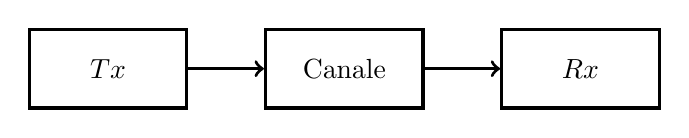
\begin{tikzpicture}[scale=2]
        \node[block](tx)at(-0.5,0){$Tx$};
        \node[block](rx)at(2.5,0){$Rx$};
        \node[block](c)at(1,0){Canale};
        \draw[->,very thick](tx.0)--(c.180);
        \draw[->,very thick](c.0)--(rx.180);
    \end{tikzpicture}
\end{center}

\subsection{Segnali a Tempo Continuo}

Vengono definiti in questa sezione una serie di segnali canonici:

\subsubsection{Seno Cardinale}

\begin{equation}
    x(t)=\mbox{sinc}(t):=\displaystyle\frac{\sin(\pi t)}{\pi t}
\end{equation}
Questo segnale si attenua asintoticamente come $1/t$: 
\begin{equation*}
    \displaystyle-\frac{1}{t}\leq\mbox{sinc}(t)\leq\frac{1}{t}
\end{equation*}
Viene incluso il fattore $\pi$ nell'argomento in modo che la funzione si annulli per ogni valore intero:
\begin{equation*}
    \mbox{sinc}(t)=0\,\forall t\in\mathbb{Z}
\end{equation*}

\begin{center}
    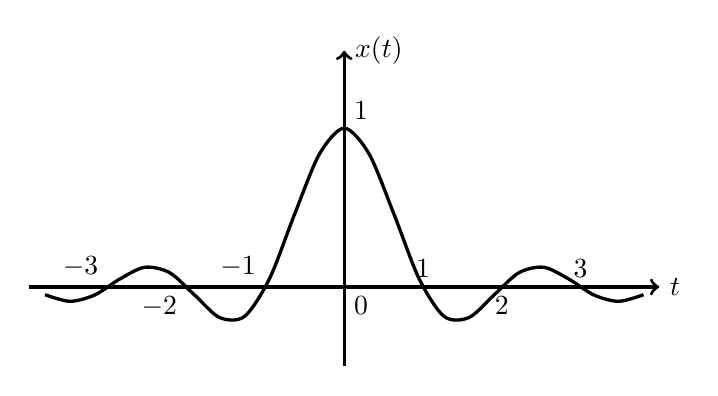
\begin{tikzpicture}[scale=2]
        \draw[->,very thick](0,-0.5)--(0,1.5)node[right]{$x(t)$};
        \draw[->,very thick](-2,0)--(2,0)node[right]{$t$};
        \draw[-,very thick]plot[smooth, domain=-1.9:1.9](\x,{1/(2*pi*\x)*sin(2*pi*\x r)});
        \node[above right]at(0,1){$1$};
        \node[above]at(0.5,0){$1$};
        \node[below]at(1,0){$2$};
        \node[above]at(1.5,0){$3$};
        \node[above left]at(-0.5,0){$-1$};
        \node[below left]at(-1,0){$-2$};
        \node[above left]at(-1.5,0){$-3$};
        \node[below right]at(0,0){$0$};

    \end{tikzpicture}
\end{center}

\subsubsection{Coseno}

\begin{equation}
    x(t)=\cos\left(\displaystyle\frac{2\pi t}{T}\right)
\end{equation}

Il parametro $T$ rappresenta il periodo della funzione, per cui il valore della funzione ad un certo valore $t$ corrisponde al valore in $t-T$. Invece del periodo si può 
usare la frequenza $f_0$, inverso del periodo. 

\begin{center}
    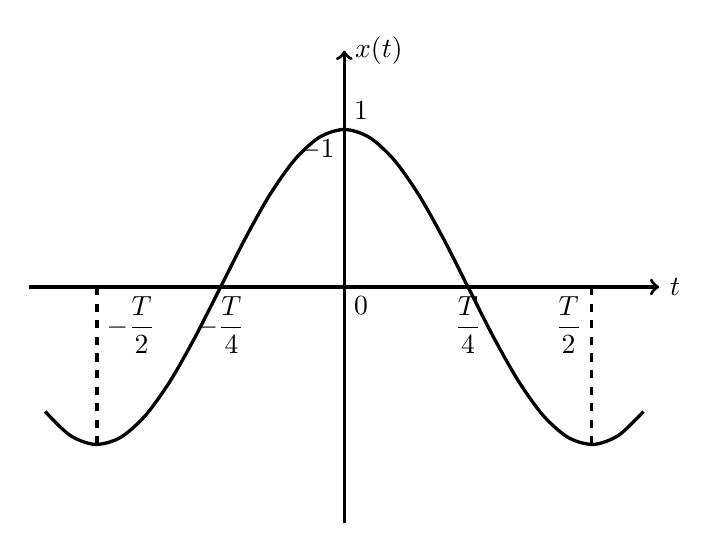
\begin{tikzpicture}[scale=2]
        \draw[->,very thick](0,-1.5)--(0,1.5)node[right]{$x(t)$};
        \draw[->,very thick](-2,0)--(2,0)node[right]{$t$};   
        \draw[-,very thick]plot[smooth, domain=-1.9:1.9](\x,{cos(2*\x r)});
        
        \node[below]at(0.785,0){$\displaystyle\frac{T}{4}$};
        \node[below]at(-0.785,0){$\displaystyle-\frac{T}{4}$};
        \node[below left]at(1.5707,0){$\displaystyle\frac{T}{2}$};
        \node[below right]at(-1.5707,0){$\displaystyle-\frac{T}{2}$};
        \draw[dashed,very thick](1.5707,0)--(1.5707,-1);
        \draw[dashed,very thick](-1.5707,0)--(-1.5707,-1);
        \node[above right]at(0,1){$1$};
        \node[below left]at(0,1){$-1$};
        \node[below right]at(0,0){$0$};
    \end{tikzpicture}
\end{center}

\subsubsection{Gradino Periodico}

\begin{center}
    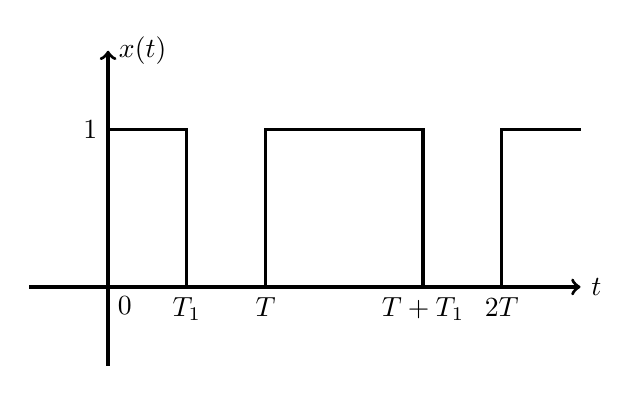
\begin{tikzpicture}[scale=2]
        \draw[->,very thick](-0.5,0)--(3,0)node[right]{$t$};
        \draw[->,very thick](0,-0.5)--(0,1.5)node[right]{$x(t)$};
        \node[below right]at(0,0){$0$};

        \draw[-,very thick](0,1)node[left]{$1$}--(0.5,1)--(0.5,0)node[below]{$T_1$}--(1,0)node[below]{$T$}--(1,1)--(2,1)--(2,0)node[below]{$T+T_1$}--(2.5,0)node[below]{$2T$}--(2.5,1)--(3,1);
    \end{tikzpicture}
\end{center}

\subsubsection{Esponenziale Complesso}

\begin{equation}
    x(t)=\displaystyle e^{i\frac{2\pi t}{T}}=\cos\left(\frac{2\pi t}{T}\right)+i\sin\left(\frac{2\pi t}{T}\right)
\end{equation}

Un segnale complesso può essere anlizzato mediante la sua fase ed il uso modulo in funzione del tempo:
\begin{equation*}
    x(t)=|x(t)|e^{\displaystyle\phase{x(t)}}
\end{equation*}

Dato che la fase è periodica si può rappresentare come una serie di rampe.

\begin{center}
    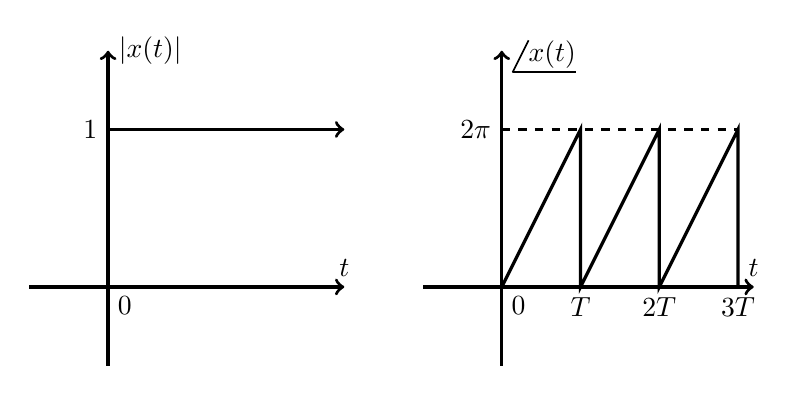
\begin{tikzpicture}[scale=2]
        \draw[->,very thick](-0.5,0)--(1.5,0)node[above]{$t$};
        \draw[->,very thick](0,1)node[left]{$1$}--(1.5,1);
        \draw[->,very thick](0,-0.5)--(0,1.5)node[right]{$|x(t)|$};
        \node[below right]at(0,0){$0$};

        \draw[->,very thick](2,0)--(4.1,0)node[above]{$t$};
        \draw[->,very thick](2.5,-0.5)--(2.5,1.5)node[right]{$\phase{x(t)}$};
        \draw[dashed,very thick](2.5,1)node[left]{$2\pi$}--(4,1);
        \node[below right]at(2.5,0){$0$};

        \draw[-,very thick](2.5,0)--(3,1)--(3,0)node[below]{$T$}--(3.5,1)--(3.5,0)node[below]{$2T$}--(4,1)--(4,0)node[below]{$3T$};
    \end{tikzpicture}
\end{center}

\subsubsection{Esponenziale}

\begin{equation}
    x(t)=e^{-\alpha t},\,\alpha\in\mathbb{R}
\end{equation}

\begin{center}
    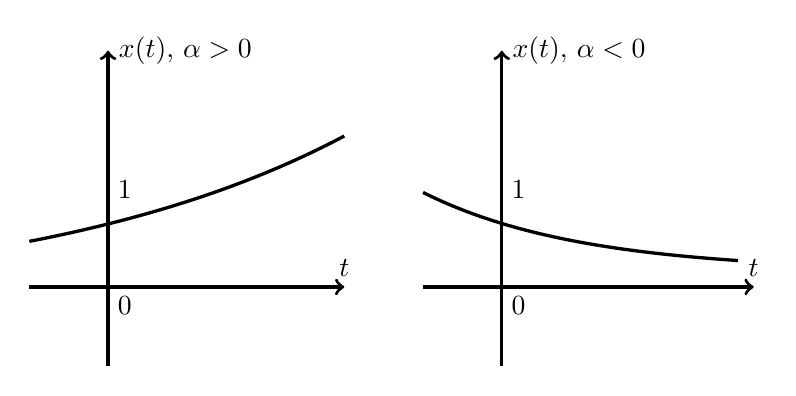
\begin{tikzpicture}[scale=2]
        \draw[->,very thick](-0.5,0)--(1.5,0)node[above]{$t$};
        \draw[->,very thick](0,-0.5)--(0,1.5)node[right]{$x(t),\,\alpha>0$};
        \draw[-,very thick]plot[smooth, domain=-0.5:1.5](\x,{1/2*e^(1/2*\x)-0.1});
        \node[above right]at(0,0.5){$1$};
        \node[below right]at(0,0){$0$};

        \draw[->,very thick](2,0)--(4.1,0)node[above]{$t$};
        \draw[->,very thick](2.5,-0.5)--(2.5,1.5)node[right]{$x(t),\,\alpha<0$};
        \draw[-,very thick]plot[smooth, domain=2:4](\x,{1/2*e^(-(\x-2))+0.1});
        \node[above right]at(2.5,0.5){$1$};
        \node[below right]at(2.5,0){$0$};
    \end{tikzpicture}
\end{center}

\subsubsection{Finestra}

\begin{equation}
    x(t)=\mbox{rect}\left(\displaystyle\frac{t}{T}\right):=\begin{cases}
        1 & \displaystyle-\frac{T}{2}\leq t <\frac{T}{2}\\
        0 & \displaystyle t<-\frac{T}{2} \land t\geq\frac{T}{2}
    \end{cases}
\end{equation}

$T$ viene chiamata base della finestra. Questo segnale presenta una discontinuità di salto per $t=\pm\displaystyle\frac{1}{2}$. La funzione finestra viene usata quando si 
vuole analizzare solo una parte di un segnale, poiché il restante sarà pari a $0$. La trasformata di questa funzione rappresenta un filtro in frequenza. 

\begin{center}
    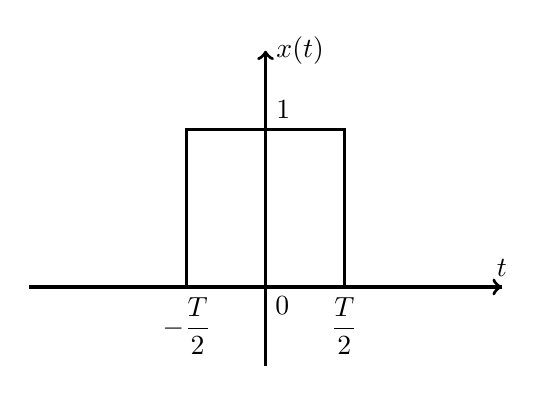
\begin{tikzpicture}[scale=2]
        \draw[->,very thick](-1.5,0)--(1.5,0)node[above]{$t$};
        \draw[->,very thick](0,-0.5)--(0,1.5)node[right]{$x(t)$};
        \node[below right]at(0,0){$0$};

        \draw[-,very thick](-1.5,0)--(-0.5,0)node[below]{$\displaystyle-\frac{T}{2}$}--(-0.5,1)--(0,1)node[above right]{$1$}--(0.5,1)--(0.5,0)node[below]{$\displaystyle\frac{T}{2}$}--(1.5,0);        
    \end{tikzpicture}
\end{center}

\subsubsection{Triangolo}

\begin{equation}
    x(t)=\mbox{tri}\left(\displaystyle\frac{t}{T}\right):=\begin{cases}
        1-|t| & -T\leq t < T\\
        0 & t<-T \land t\geq T
    \end{cases}
\end{equation}

\begin{center}
    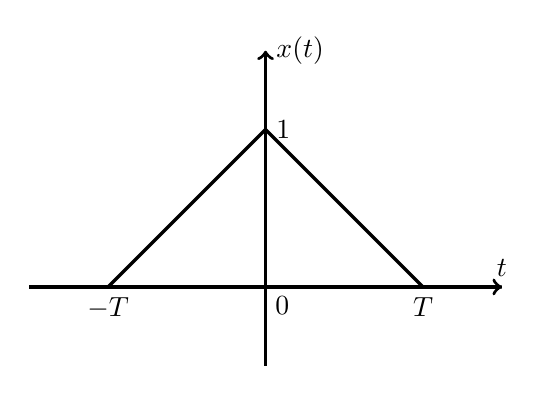
\begin{tikzpicture}[scale=2]
        \draw[->,very thick](-1.5,0)--(1.5,0)node[above]{$t$};
        \draw[->,very thick](0,-0.5)--(0,1.5)node[right]{$x(t)$};
        \node[below right]at(0,0){$0$};

        \draw[-,very thick](-1.5,0)--(-1,0)node[below]{$-T$}--(0,1)node[right]{$1$}--(1,0)node[below]{$T$}--(1.5,0);
    \end{tikzpicture}
\end{center}

\subsubsection{Gradino}

\begin{equation}
    x(t)=u(t):=\begin{cases}
        1 & t\geq0\\
        0 & t<0
    \end{cases}
\end{equation}

\begin{center}
    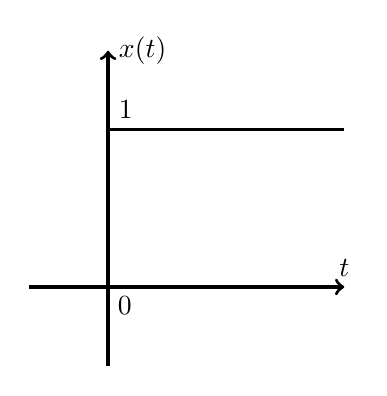
\begin{tikzpicture}[scale=2]
        \draw[->,very thick](-0.5,0)--(1.5,0)node[above]{$t$};
        \draw[->,very thick](0,-0.5)--(0,1.5)node[right]{$x(t)$};
        \draw[-,very thick](-0.5,0)--(0,0)--(0,1)node[above right]{$1$}--(1.5,1);
        \node[below right]at(0,0){$0$};
    \end{tikzpicture}
\end{center}

\subsubsection{Gaussiana}

\begin{equation*}
    x(t)=e^{-\alpha t^2}\,\,\alpha\in\mathbb{R}^+
\end{equation*}

La larghezza della campana centrale dipende dal fattore $\alpha$. Nello sturio delle probabiltà, si usa la sua forma normalizzata:
\begin{equation*}
    x(t)=\displaystyle\frac{e^{-\frac{t^2}{2\sigma^2}}}{\sqrt{2\pi}\sigma}
\end{equation*}
Il valore $\sigma$ rappresenta la deviazione standard, mentre il suo quadrato $\sigma^2$ descrive la varianza. 

\begin{center}
    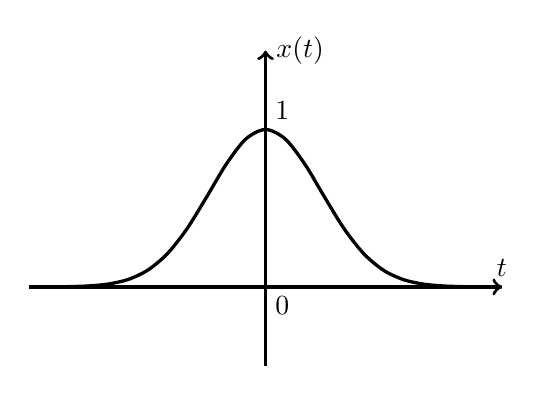
\begin{tikzpicture}[scale=2]
        \draw[->,very thick](-1.5,0)--(1.5,0)node[above]{$t$};
        \draw[->,very thick](0,-0.5)--(0,1.5)node[right]{$x(t)$};
        \node[below right]at(0,0){$0$};
        \node[above right]at(0,1){$1$};


        \draw[-,very thick]plot[smooth, domain=-1.5:1.5](\x,{e^(-(2*\x)^2)});
    \end{tikzpicture}
\end{center}

\subsubsection{Esponenziale Unilatero}

\begin{equation*}
    x(t)=e^{-\alpha t}\cdot u(t)\,\,\alpha\in\mathbb{R}^+
\end{equation*}

\begin{center}
    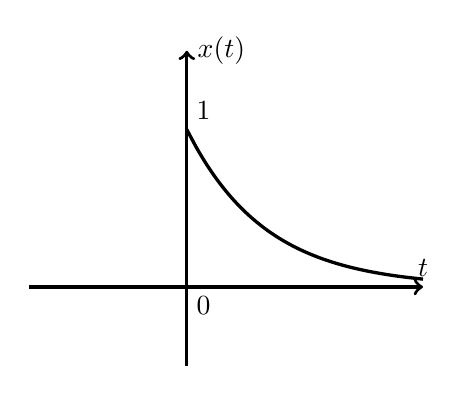
\begin{tikzpicture}[scale=2]
        \draw[->,very thick](-1,0)--(1.5,0)node[above]{$t$};
        \draw[->,very thick](0,-0.5)--(0,1.5)node[right]{$x(t)$};
        \node[below right]at(0,0){$0$};
        \node[above right]at(0,1){$1$};

        \draw[-,very thick](-1,0)--(0,0);
        \draw[-,very thick]plot[smooth, domain=0:1.5](\x,{e^(-2*(\x))});
    \end{tikzpicture}
\end{center}

\subsubsection{Costante}

\begin{equation*}
    x(t)=a
\end{equation*}

\begin{center}
    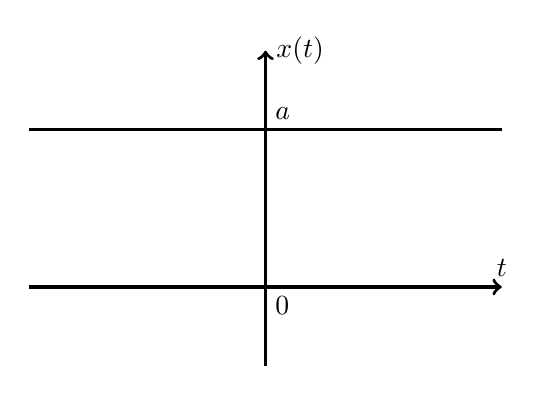
\begin{tikzpicture}[scale=2]
        \draw[->,very thick](-1.5,0)--(1.5,0)node[above]{$t$};
        \draw[->,very thick](0,-0.5)--(0,1.5)node[right]{$x(t)$};
        \node[below right]at(0,0){$0$};
        \node[above right]at(0,1){$a$};

        \draw[-,very thick](-1.5,1)--(1.5,1);
    \end{tikzpicture}
\end{center}

\subsubsection{Segno}

\begin{equation*}
    x(t)=\mbox{sign}(t):=\begin{cases}
        1&t>0\\
        -1&t<0
    \end{cases}
\end{equation*}

\begin{center}
    \begin{tikzpicture}[scale=2]
        \draw[->,very thick](-1.5,0)--(1.5,0)node[above]{$t$};
        \draw[->,very thick](0,-1.5)--(0,1.5)node[right]{$x(t)$};
        \node[below right]at(0,0){$0$};
        \node[above right]at(0,1){$1$};
        \node[below left]at(0,-1){$-1$};

        \draw[-,very thick](0,1)--(1.5,1);
        \draw[-,very thick](0,-1)--(-1.5,-1);
    \end{tikzpicture}
\end{center}

\subsection{Operazioni sui Segnali}

Le operazioni sui segnali vengono computate istante per istante. L'operazione di somma produce un segnale $z(t)$, tale che ogni valore che assume equivale alla somma 
di altri due segnali $x(t)$ e $y(t)$ nello stesso istante:
\begin{equation*}
    z(t)=x(t)+y(t)
\end{equation*}

Analogamente si considera l'operazione prodotto, come un prodotto istante per istante tra i due segnali:
\begin{equation*}
    z(t)=x(t)\cdot y(t)
\end{equation*}

L'operazione di ribaltamento corrisponde ad una riflessione della funzione lungo l'asse delle ascisse di un segnale $x(t)$ tramite una sostituzione di variabile $t\to-t$:
\begin{equation*}
    z(t)=x(-t)
\end{equation*}
Quest'operazione non produce risultati per segnali pari, poiché presentano la proprietà $x(t)=x(-t)$. 
Tramite l'operazione di ribaltamento si può esprimere il segnale segno tramite la differenza di due gradini:
\begin{equation*}
    \mbox{sign}(t)=u(t)-u(-t)
\end{equation*}


L'operazione di traslazione, sposta un segnale $x(t)$ lungo l'asse delle ascisse di un fattore $\tau$:
\begin{equation*}
    z(t)=x(t-\tau)
\end{equation*}

L'operazione di cambio di scale corrisponde ad un rimpicciolimento o allargamento di un segnale $x(t)$ di un fattore $a\in\mathbb{R}$:
\begin{equation*}
    z(t)=x(at)
\end{equation*}

\subsection{Energia e Potenza}

L'energia e la potenza di un segnale rappresentano caratteristiche utili nella loro analisi e processazione. 

Viene definita energia $E_x$ di un segnale $x(t)$, come il limite per $\Delta t\to0$ di un integrale:
\begin{equation}
    E_x:=\lim_{\Delta t\to\infty}\displaystyle\int_{-\frac{\Delta t}{2}}^{\frac{\Delta t}{2}}|x(t)|^2dt=\int_{-\infty}^{\infty}|x(t)|^2dt
\end{equation}
L'energia di un segnale è sempre strettamente positiva, poiché si considera tutta l'area sottesa dal quadrato del modulo del segnale, necessariamente positivo; mentre è nulla 
solo se lo è anche il segnale analizzato. Teoricamente non esiste un limite per l'energia contenuta in un segnale, ma sono fisicamente realizzabile solo segnali con energia 
finita e non infinita. 

Se l'energia di un segnale è finita e diversa da zero $E_x\neq\infty$ e $E_x\neq0$, il segnale $x(t)$ si chiama segnale di energia.


Viene definita la potenza $P_x$ di un segnale $x(t)$ in maniera simile alla sua energia:
\begin{equation}
    P_x:=\lim_{\Delta t\to\infty}\displaystyle\left(\frac{1}{\Delta t}\int_{-\frac{\Delta t}{2}}^{\frac{\Delta t}{2}}|x(t)|^2dt\right)
\end{equation}
Anche la potenza di un segnale è strettamente positiva $P_x\geq0$, se la potenza assume valori diversi da zero e finiti, il segnale $x(t)$ si chiama segnale di potenza. 

Vengono così create due classi di segnali, di potenza e di energi. Per la definizione delle due grandezze antisimmetriche poiché se un segnale è di potenza, non è di energia 
e viceversa: 
\begin{gather*}
    E\implies\neg P\\
    P\implies\neg E
\end{gather*}

Si determina l'energia di una gaussiana di ampiezza $A$:
\begin{gather*}
    E_x=\lim_{\Delta t\to\infty}\displaystyle\int_{-\frac{\Delta t}{2}}^{\frac{\Delta t}{2}}A^2e^{-2\alpha t^2}dt=A^2\lim_{\Delta t\to\infty}\displaystyle\int_{-\frac{\Delta t}{2}}^{\frac{\Delta t}{2}}e^{-2\alpha t^2}dt
\end{gather*}
Si considera il cambio di variabile $\tau=\sqrt{2\alpha}t$:
\begin{equation*}
    E_x=A^2\lim_{\Delta t\to\infty}\displaystyle\int_{-\frac{\Delta t}{2}}^{\frac{\Delta t}{2}}\frac{e^{-\tau^2}}{\sqrt{2\alpha}}d\tau=\frac{A^2}{\sqrt{2\alpha}}\int_{-\infty}^{+\infty}e^{-\tau^2}d\tau
\end{equation*}

L'integrale ottenuto è l'integrale di Gauss, risolubile applicando un cambio di coordinate polari al quadrato dell'integrale dato, il risultato dell'integrazione della 
gaussiana sull'intero asse dei reali $\mathbb{R}$ corrisponde alla radice di pi greco: 
\begin{equation*}
    \displaystyle\int_{\mathbb{R}}e^{-t^2}dt=\sqrt\pi
\end{equation*}
Per cui l'energia di una gaussiana risulta essere:
\begin{equation}
    E_x=A^2\displaystyle\sqrt{\frac{\pi}{2\alpha}}
\end{equation}




Moltiplicando un segnale $x(t)$ moltiplicato per un gradino e calcolandone l'integrale sui tutti i reali $\mathbb{R}$, equivale all'integrale del segnale originiario sui soli 
reali positivi $\mathbb{R}^+$, poiché il segnale assume valori nulli da $-\infty$ a $0$: 
\begin{equation*}
    \displaystyle\int_{\mathbb{R}}x(t)\cdot u(t)dt=\int_{\mathbb{R}^+}x(t)dt
\end{equation*}



Si determina l'energia e la potenza di un esponenziale complesso. Il segnale ha un modulo unitario $|x(t)|=1$, per cui la sua energia risultante è:
\begin{equation*}
    E_x=\lim_{\Delta t\to\infty}\displaystyle\int_{-\frac{\Delta t}{2}}^{\frac{\Delta t}{2}}dt=\lim_{\Delta t\to\infty}\left(\frac{\Delta t}{2}+\frac{\Delta t}{2}\right)=\infty
\end{equation*}
Per cui l'esponenziale complesso non è un segnale di energia. La potenza risulta essere:
\begin{equation*}
    P_x=\lim_{\Delta t\to\infty}\displaystyle\left(\frac{1}{\Delta t}\int_{-\frac{\Delta t}{2}}^{\frac{\Delta t}{2}}dt\right)=\lim_{\Delta t\to\infty}\left(\frac{1}{\Delta t}\cdot\Delta t\right)=1
\end{equation*}
L'esponenziale complesso è quindi un segnale di potenza. 



Si determina l'energia di un esponenziale unilatero:
\begin{equation*}
    E_x=\displaystyle\int_{\mathbb{R}^+}e^{-2\alpha t}dt=\frac{1}{2\alpha}
\end{equation*}
Per cui questo segnale non è né di energia né di potenza. 


I segnali periodici non possono essere di energia, per cui un segnale perdiodico senza attenuazione non è fisicamente realizzabile. Quindi possono essere solo di potenza, 
si determina la potenza di un segnale periodico:
\begin{equation*}
    P_x=\lim_{\Delta t\to\infty}\displaystyle\left(\frac{1}{\Delta t}\int_{-\frac{\Delta t}{2}}^{\frac{\Delta t}{2}}|x(t)|^2dt\right)
\end{equation*}
In un segnale periodico si può esprimere l'intervallo di tempo $\Delta t$ come $n$ volte il periodo $T$:
\begin{equation*}
    P_x=\lim_{n\to\infty}\displaystyle\left(\frac{1}{n T}\int_{-\frac{nT}{2}}^{\frac{nT}{2}}|x(t)|^2dt\right)
\end{equation*}
L'integrale di un segnale perfettamente periodico, ovvero senza smorzamenti, su $n$ periodi equivale ad $n$ volte l'integrale su un singolo periodo $T$:
\begin{equation*}
    P_x=\lim_{n\to\infty}\displaystyle\left(\frac{1}{n T}n\int_{-\frac{n}{2}}^{\frac{T}{2}}|x(t)|^2dt\right)=\lim_{n\to\infty}\displaystyle\left(\frac{1}{T}\int_{-\frac{T}{2}}^{\frac{T}{2}}|x(t)|^2dt\right)
\end{equation*} 
Questo integrale è indipendente dalla variabile $n$, per cui si può trascurare il limite, la potenza risulta quindi essere:
\begin{equation}
    P_x=\displaystyle\frac{1}{T}\int_{-\frac{T}{2}}^{\frac{T}{2}}|x(t)|^2dt
\end{equation}
Quest'ultimo integrale può essere espresso in termini della frequenza naturale: $f_0=\frac{1}{T}$. 



Si determina la potenza del segnale coseno, di ampiezza $A$ e frequenza naturale $f_0$ $A\cos\left(2\pi f_0t\right)$:
\begin{equation*}
    P_x=\displaystyle A^2f_0\int_{-\frac{1}{2f_0}}^{\frac{1}{2f_0}}\cos^2(2\pi f_0 t)dt
\end{equation*}
Per esprimere il quadrato del coseno, si consdira la formula di bisezione del coseno:
\begin{gather*}
    \cos(2x)=2\cos^2(x)-1\\
    \cos^2(x)=\displaystyle\frac{\cos(2x)+1}{2}
\end{gather*}
Si può esprimere inoltre mediante la notazione complessa delle funzioni trigonometriche. 
Considerando questa sostituzione, l'integrale diventa:
\begin{equation*}
    P_x=\displaystyle\frac{A^2f_0}{2}\int_{-\frac{1}{2f_0}}^{\frac{1}{2f_0}}(\cancelto{0}{\cos(4\pi f_0 t)}+1)dt=\frac{A^2f_0}{2}\left(\frac{1}{2f_0}+\frac{1}{2f_0}\right)=\frac{A^2}{2}
\end{equation*}
L'integrale su un periodo del coseno è nullo, poiché è una funzione pari, per cui la componente $\cos(4\pi f_0 t)$ fornisce un contributo nullo. 

\end{document}
